% !TEX root = ../main.tex
\section{Дискретні випадкові вектори}
\begin{definition}
    Вимірна функція $\Omega \mapsto \mathbb{R}^n$, задана на ймовірнісному 
    просторі $\left\{\Omega, \mathcal{F}, P \right\}$, 
    називається \emph{випадковим вектором (системою випадкових величин)}.
    Позначається
$\vec{\xi} = \vec{\xi}(\omega) = 
\left(\xi_1(\omega), \xi_2(\omega), ... , \xi_n(\omega)\right)^{T}$.
\end{definition}

\begin{remark}
    Під вимірністю мається на увазі те, що 
    \begin{equation*}
        \forall \vec{x} \in \mathbb{R}^n: 
        A=\left\{\omega \in \Omega: \xi_1(\omega) < x_1, 
                                    \xi_2(\omega) < x_2,
                                    ... ,
                                    \xi_n(\omega) < x_n\right\}
        \in \mathcal{F}
    \end{equation*}
\end{remark}

\begin{definition}
    Випадковий вектор називається \emph{дискретним}, якщо всі його координати --- 
    дискретні випадкові величини.
\end{definition}
\begin{remark}
    Випадковий вектор можна трактувати як випадкову точку в $\mathbb{R}^n$.
    При $n = 2$: $\vec{\xi} = (\xi_1, \xi_2)^T$ --- випадкова точка на площині. 
\end{remark}

Закон розподілу двовимірного дискретного випадкового вектора задається 
\emph{таблицею розподілу}.


\hbox to \hsize{\hfil{
\begin{tabular}{c c}
    \begin{tabular}{|c|c|c|c|c|}
        \hline
        \diagbox{$\xi_2$}{$\xi_1$} & $x_1$ & $x_2$ & ... & $x_n$ \\
        \hline
        $y_1$ & $p_{11}$ & $p_{21}$ & ... & $p_{n1}$ \\
        \hline
        $y_2$ & $p_{12}$ & $p_{22}$ & ... & $p_{n2}$ \\
        \hline
        ... & ... & ... & $p_{ij}$ & ... \\
        \hline
        $y_m$ & $p_{1m}$ & $p_{2m}$ & ... & $p_{nm}$ \\
        \hline
    \end{tabular} &
    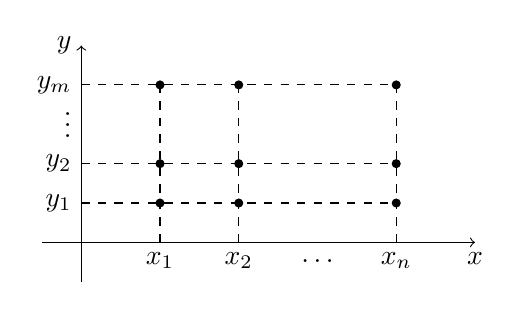
\begin{tikzpicture}[baseline={(current bounding box.center)}]
        \draw [->] (-0.5, 0) -- (5, 0); 
        \draw [->] (0, -0.5) -- (0, 2.5);
        %\draw [fill] (1, 1) circle [radius = 0.05];
        \foreach \i in {1,...,2}:
            %\draw [dashed] (\i, 0) -- (\i, 1.5);
            \foreach \j in {1,...,2}:
                \draw [fill] (\i, {\j/2}) circle [radius = 0.05];
        \foreach \k in {1,...,2} {
            \draw [fill] (4, {\k/2}) circle [radius = 0.05];
            \draw [fill] (\k, 2) circle [radius = 0.05];
            \draw [dashed] (\k, 0) -- (\k, 2);
            \node [below] at (\k, 0) {$x_\k$};
            \node [left] at (0, {\k/2}) {$y_\k$};
            \draw [dashed] (0, {\k/2}) -- (4, {\k/2});
        }
        \draw [fill] (4, 2) circle [radius = 0.05];
        \draw [dashed] (4, 0) -- (4, 2);
        \node [below] at (3, -0.1) {$\ldots$};
        \node [below] at (4, 0) {$x_n$};
        \node [below] at (5, 0) {$x$};
        \draw [dashed] (0, 2) -- (4, 2);
        \node [left] at (0, 1.6) {$\vdots$};
        \node [left] at (0, 2) {$y_m$};
        \node [left] at (0, 2.5) {$y$};
    \end{tikzpicture}
\end{tabular}
}\hfil}
$p_{ij} = P\left\{\xi_1 = x_i, \xi_2 = y_m\right\}$, $\sum\limits_{i,j} p_{ij} = 1$.

З таблиці розподілу можна обчислити ряди розподілу $\xi_1$ та $\xi_2$:

\hbox to \hsize{\hfil{
    \begin{tabular}{c c}
        \begin{tabular}{c|c|c|c|c}
            $\xi_1$ & $x_1$ & $x_2$ & ... & $x_n$ \\
            \hline
            $p$ & $\sum\limits_{k=1}^m p_{1k}$ & $\sum\limits_{k=1}^m p_{2k}$ & ... & $\sum\limits_{k=1}^m p_{nk}$
        \end{tabular} &
        \begin{tabular}{c|c|c|c|c}
            $\xi_2$ & $y_1$ & $y_2$ & ... & $y_m$ \\
            \hline
            $p$ & $\sum\limits_{k=1}^n p_{k1}$ & $\sum\limits_{k=1}^n p_{k2}$ & ... & $\sum\limits_{k=1}^n p_{km}$
        \end{tabular}
    \end{tabular}
}\hfil}

\begin{remark}
    Обчислити таблицю розподілу, знаючи ряди розподілу координат, можна лише у випадку їх незалежності.
\end{remark}

\subsection{Сумісна функція розподілу двовимірного випадкового вектору}
\begin{definition} 
    \emph{Сумісною функцією розподілу} двовимірного випадкового вектора $\vec{\xi}$ 
    називається $F_{\vec{\xi}}(x, y) = P\left\{\omega: \xi_1 < x,\; \xi_2 < y\right\} = 
    P(\xi_1 < x, \; \xi_2 < y)$
\end{definition}

\textbf{Геометрична інтерпретація: }
Значення $F_{\vec{\xi}}(x, y)$ рівне імовірності 
потрапляння точки в заштриховану зону.

\hbox to \hsize{\hfil{
    \begin{tikzpicture}
        \draw [->] (-0.5, 0) -- (3, 0);
        \draw [->] (0, -0.5) -- (0, 3);
        \draw [fill] (2, 2) circle [radius=0.05];
        \node [above right] at (2, 2) {$(x, y)$};
        \path [pattern=north west lines, 
                pattern color=gray] (2, 2) rectangle (-0.55, -0.51);
        \draw [dashed] (-0.5, 2) -- (2, 2) -- (2, -0.5);
        \node [below] at (3, 0) {$x$};
        \node [above right] at (0.2, 0.2) {$F_{\vec{\xi}}(x, y)$};
        \node [left] at (0, 3) {$y$};
    \end{tikzpicture}
}\hfil}

\noindent\textbf{Властивості: }
\begin{enumerate}
    \item $D(F_{\vec{\xi}}) = \mathbb{R}^2$, $E(F_{\vec{\xi}}) = 
    \left<0, 1\right>$.
    \item Монотонно неспадна по кожній з координат.
    \begin{proof}
        $A = \left\{\xi_1 < x_2,\;\xi_2 < y \right\}$, 
        $B = \left\{x_2 \leq \xi_1 < x_1,\; \xi_2<y\right\}$, 
        $C = \left\{\xi_1 < x_1,\; \xi_2 < y\right\}$.

        $C = A \vee B \Rightarrow P(C) = P(A) + P(B)$
    
        $P(C) = F_{\vec{\xi}}(x_1, y)$,  
        $P(A) = F_{\vec{\xi}}(x_2, y)$

        $F_{\vec{\xi}}(x_1, y) = F_{\vec{\xi}}(x_2, y) + P(B)
        \Rightarrow F_{\vec{\xi}}(x_1, y) \geq  F_{\vec{\xi}}(x_2, y)$. 
        
        Для другої координати аналогічно.
    \end{proof}
    \item $\lim\limits_{x \to -\infty} F_{\vec{\xi}}(x, y) = 
           \lim\limits_{y \to -\infty} F_{\vec{\xi}}(x, y) = 
           \lim\limits_{x,y \to -\infty} F_{\vec{\xi}}(x, y) = 0$.
    \begin{proof}
        Строге доведення ґрунтується на теоремах про неперервність 
        ймовірності.

        $\lim\limits_{x \to -\infty} F_{\vec{\xi}}(x, y) = 
        \lim\limits_{x \to -\infty} P\left\{\xi_1<x,\;\xi_2<y\right\} 
        = [\text{використаємо теорему про неперервність}$ 
        $\text{ймовірності}] = P(\varnothing \cap \{\xi_2 < y\})
        = P(\varnothing) = 0$.
        Інші випадки --- аналогічно.
    \end{proof}
    \item \emph{<<Умови узгодженості>>}
    
    $\lim\limits_{x \to +\infty} F_{\vec{\xi}}(x, y) = F_{\xi_2}(y)$, 
    $\lim\limits_{y \to +\infty} F_{\vec{\xi}}(x, y) = F_{\xi_1}(x)$
    \begin{proof}
        $\lim\limits_{x \to +\infty} F_{\vec{\xi}}(x, y) = 
        \lim\limits_{x \to +\infty} 
        P\left(\xi_1 < x,\; \xi_2 < y\right) = 
        P\left(\xi_1 < +\infty,\;\xi_2<y\right) = $
        
        $= P\left(\xi_2<y\right) = F_{\xi_2}(y)$. Інша - аналогічно.
    \end{proof}
    \item $\lim\limits_{x,y \to +\infty} F_{\vec{\xi}}(x, y) = 1$
    \begin{proof}
        Напряму випливає з умов узгодженості.
    \end{proof}
    \item Функція розподілу є неперервною зліва по кожному з аргументів: 
    
    $\lim\limits_{x \to x_0 - 0} F_{\vec{\xi}}(x, y) = F_{\vec{\xi}}(x_0, y)$, 
    $\lim\limits_{y \to y_0 - 0} F_{\vec{\xi}}(x, y) = F_{\vec{\xi}}(x, y_0)$.
    \begin{proof}
        Аналогічне доведення з одновимірним випадком (твердж. \refeq{2_1_con}, 
        с. \pageref{2_1_con}).
    \end{proof}
    \item $P\left(\vec{\xi} \in \Pi \right)$ - ?
\suspend{enumerate}